\documentclass[11pt,a4paper]{article}
\usepackage[margin=2.5cm]{geometry}
\usepackage{amsmath,amssymb}
\usepackage{booktabs}
\usepackage{array}
\usepackage{xcolor}
\usepackage{tcolorbox}
\tcbuselibrary{skins,breakable}
\usepackage{hyperref}
\usepackage[numbers,sort&compress]{natbib}
\bibliographystyle{unsrtnat}
\hypersetup{colorlinks=true,linkcolor=blue!60!black,urlcolor=blue!60!black}
\usepackage{tikz}
\usetikzlibrary{shapes.geometric,arrows.meta,positioning,calc,decorations.pathmorphing}
\usepackage{enumitem}

\definecolor{boxblue}{RGB}{220,235,255}
\definecolor{boxorange}{RGB}{255,240,210}
\definecolor{boxgreen}{RGB}{220,245,220}
\definecolor{boxyellow}{RGB}{255,252,210}

\newcommand{\term}[1]{\textbf{#1}}
\newcommand{\lean}[1]{\texttt{#1}}

\title{\textbf{Why the Strong CP Problem Is Solved:}\\[6pt]
\large $\theta_{\mathrm{QCD}} = 0$ from $F_{21}$ Group Theory\\[4pt]\normalsize\textit{UGP Physics Tutorial Series}
\\[2pt]\small\href{https://doi.org/\TutorialDOI}{doi.org/\TutorialDOI}}
\author{Nova Spivack\\[4pt]
\normalsize
\href{https://novaspivack.com/research}{novaspivack.com/research}\\[2pt]
\small Full monograph (P48):
\href{https://doi.org/10.5281/zenodo.20560550}{doi.org/10.5281/zenodo.20560550}
}
\newcommand{\TutorialDOI}{10.5281/zenodo.20657902}
\date{2026}

\begin{document}
\setcounter{tocdepth}{2}
\maketitle
\tableofcontents
\newpage

\begin{tcolorbox}[colback=blue!6,colframe=blue!40!black,
  title=\textbf{UGP Physics Tutorial Series}]
\textbf{Prerequisites (read first):} \href{https://doi.org/10.5281/zenodo.20657898}{\emph{How the Standard Model Quantum Numbers Emerge}} $\cdot$ \href{https://doi.org/10.5281/zenodo.20657889}{\emph{The GTE Polynomial: A Step-by-Step Cheat Sheet}}\\[4pt]
\textbf{See also:} \href{https://doi.org/10.5281/zenodo.20657923}{\emph{The Weinberg Angle, Fine-Structure Constant, and Gauge Couplings}} $\cdot$ \href{https://doi.org/10.5281/zenodo.20657898}{\emph{How the Standard Model Quantum Numbers Emerge}}
\end{tcolorbox}

\begin{tcolorbox}[colback=boxgreen,colframe=green!50!black,
  title=\textbf{Claim-Strength Taxonomy}]
Throughout this tutorial, results are labeled with a confidence grade:
\begin{itemize}[itemsep=2pt]
  \item \textbf{$\mathbf{A}_{\rm Lean}$ (CatAL)} --- Machine-certified in Lean~4 with zero \texttt{sorry} and zero custom axioms.  Independently verifiable by anyone with Lean installed.
  \item \textbf{A/D (CatAD)} --- Analytically derived with full derivation, computationally confirmed.  Not yet machine-certified.
  \item \textbf{A (CatA)} --- Analytically derived; derivation complete but not independently machine-certified.
  \item \textbf{A/D (conditional)} --- Derived under a named, stated premise; the premise is itself an open problem or a CatB assumption.
  \item \textbf{B (CatB)} --- A stated working hypothesis or structural premise; not yet derived.
\end{itemize}
\end{tcolorbox}


%─────────────────────────────────────────────────────────────────────────────
\section{The Strong Force: A Brief Orientation}
%─────────────────────────────────────────────────────────────────────────────

\begin{tcolorbox}[colback=boxblue,colframe=blue!40!black,title=In one sentence]
The strong force is the force that holds protons and neutrons together inside the nucleus of every atom --- and it has a deep mystery hiding inside its mathematical description.
\end{tcolorbox}

\subsection{What is the strong force?}

Every atom has a nucleus at its centre.  The nucleus contains protons and neutrons, packed tightly together.  But protons carry positive electric charge, and like charges repel.  Something must overcome that repulsion --- otherwise every nucleus would fly apart instantly.  That something is the \term{strong force}, also called the \term{strong nuclear force}.

The strong force is carried by particles called \term{gluons}, and the ``charge'' it acts on is called \term{colour charge} (nothing to do with visible colour --- it is just a name for a quantum number).  There are three types of colour charge, called red, green, and blue by convention.  Quarks carry colour charge; protons and neutrons are each made of three quarks, one of each colour.  The strong force between colour charges is far more powerful than electromagnetism at short distances, which is why it wins the battle and keeps the nucleus intact.

The \term{Standard Model of particle physics} describes the strong force using a mathematical framework called \term{Quantum Chromodynamics} (QCD).  QCD has been tested to extraordinary precision and is one of the most successful theories in all of science.

\subsection{What is a Lagrangian?}

Before we can describe the mystery, we need one more concept.  A \term{Lagrangian} is a mathematical object --- a function of the fields in a theory --- that encodes all the dynamics.  You can think of it as the ``recipe'' from which all the equations of motion are derived.  If you know the Lagrangian, you know how every field evolves and how particles interact.

The QCD Lagrangian is the recipe for the strong force.  It tells you how quarks and gluons interact.

%─────────────────────────────────────────────────────────────────────────────
\section{The Strong CP Problem}
%─────────────────────────────────────────────────────────────────────────────

\begin{tcolorbox}[colback=boxorange,colframe=orange!60!black,title=The mystery in one sentence]
The QCD Lagrangian legally allows a term that would make the neutron act like a tiny bar magnet --- but experiments show the neutron is, to extraordinary precision, \emph{not} a bar magnet.  Nobody knows why.
\end{tcolorbox}

\subsection{CP symmetry and why it matters}

Two important symmetries of physics are:
\begin{itemize}
  \item \textbf{C (charge conjugation):} replace every particle with its antiparticle.
  \item \textbf{P (parity):} flip space left-to-right, like looking in a mirror.
\end{itemize}

The combined symmetry \term{CP} is the operation of doing both at once.  Many physical processes are symmetric under CP: a process and its CP-mirror image happen at the same rate.  CP \term{violation} --- when the two rates differ --- has been observed in the weak force but is expected to be negligibly small in the strong force.

\subsection{The $\theta$ term}

The QCD Lagrangian contains all the terms that are allowed by the symmetries of the strong force.  Most of these terms are constrained to be there.  But there is one term that is \emph{allowed but not forced} --- a term that can be anything:

\begin{tcolorbox}[colback=boxyellow,colframe=yellow!60!black,title=The theta term in QCD]
\[
  \mathcal{L}_\theta \;=\; \theta_{\mathrm{QCD}}
  \cdot \frac{g_s^2}{32\pi^2} \,
  \mathrm{tr}\!\left(F^{\mu\nu}\tilde{F}_{\mu\nu}\right)
\]
\begin{center}
\small $\theta_{\mathrm{QCD}}$ is a free parameter that can take any value from $0$ to $2\pi$.\\
$F^{\mu\nu}$ is the gluon field strength; $\tilde{F}_{\mu\nu}$ is its dual (a rotated version).
\end{center}
\end{tcolorbox}

This term violates \textbf{CP symmetry} in the strong force.  The larger $|\theta_{\mathrm{QCD}}|$ is, the more the strong force violates CP.

\subsection{The neutron electric dipole moment}

If the strong force violates CP, then the neutron --- which is built from quarks glued together by the strong force --- will develop an \term{electric dipole moment}: it will act like a tiny bar magnet with a positive end and a negative end.  The size of this dipole moment is directly proportional to $|\theta_{\mathrm{QCD}}|$.

Decades of precise experiments have measured the neutron electric dipole moment.  The result:

\begin{center}
\begin{tabular}{lll}
\toprule
Quantity & Measurement & Implication \\
\midrule
Neutron EDM & $<\!1.8\times10^{-26}$ $e\cdot$cm & Consistent with zero \\
Corresponding bound on $|\theta_{\mathrm{QCD}}|$ & $<10^{-10}$ & Extremely small \\
Allowed range by QCD alone & $[0,\;2\pi)$ & No restriction \\
\bottomrule
\end{tabular}
\end{center}

\medskip
The parameter $\theta_{\mathrm{QCD}}$ could in principle be any number between 0 and $2\pi \approx 6.28$.  Yet experiments tell us it is smaller than $10^{-10}$ --- a number so close to zero it is almost incomprehensible.  If you picked a random number between 0 and 6, the chance of it being smaller than $10^{-10}$ is one in 60 billion.

\subsection{The pencil on its tip}

\begin{tcolorbox}[colback=boxgreen,colframe=green!50!black,title=Analogy: the balanced pencil]
Imagine balancing a pencil on its tip.  It could fall in any direction.  If you found a pencil that had been perfectly balanced on its tip for the entire history of the universe, you would want to know \emph{why}.  Just saying ``it happened to balance'' is not a satisfying answer.  You would expect some physical mechanism keeping it there.

The strong CP problem is the pencil: $\theta_{\mathrm{QCD}}$ is balanced at zero to ten decimal places.  Standard physics has no explanation for this balance.
\end{tcolorbox}

This is the \term{strong CP problem}: why is $\theta_{\mathrm{QCD}}$ so close to zero?  The Standard Model gives no answer.  It is one of the deepest unsolved problems in particle physics.

%─────────────────────────────────────────────────────────────────────────────
\section{The Standard Solution: Axions}
%─────────────────────────────────────────────────────────────────────────────

\begin{tcolorbox}[colback=boxblue,colframe=blue!40!black,title=The axion idea]
In 1977, Roberto Peccei and Helen Quinn proposed a solution: add a new symmetry to the theory, which spontaneously breaks and produces a new particle (the \term{axion}).  The axion dynamically adjusts its value to relax $\theta_{\mathrm{QCD}}$ to zero, like a ball rolling to the bottom of a bowl.
\end{tcolorbox}

\subsection{How Peccei--Quinn symmetry works}

The Peccei--Quinn (PQ) mechanism works in three steps:
\begin{enumerate}
  \item Introduce a new global symmetry $\mathrm{U}(1)_{\mathrm{PQ}}$.
  \item This symmetry spontaneously breaks at some high energy scale $f_a$.
  \item By Goldstone's theorem, the breaking produces a new pseudo-Nambu--Goldstone boson: the \term{axion} $a(x)$.
\end{enumerate}

Crucially, the axion couples to the same $F^{\mu\nu}\tilde{F}_{\mu\nu}$ combination that appears in the $\theta$ term.  The effective theta becomes:
\[
  \theta_{\mathrm{eff}} \;=\; \theta_{\mathrm{QCD}} + \frac{a(x)}{f_a}.
\]
At its minimum energy, the axion field settles at the value $a/f_a = -\theta_{\mathrm{QCD}}$, cancelling the $\theta$ term exactly.  The pencil falls to $\theta_{\mathrm{eff}} = 0$.

\subsection{The problem with axions}

The PQ mechanism is elegant, but it has a fundamental issue: it solves one mystery by inventing a new particle that has never been observed.

\begin{center}
\begin{tabular}{@{}p{3.2cm}p{9cm}@{}}
\toprule
Issue & Detail \\
\midrule
Not yet found & Dedicated experiments (ADMX, HAYSTAC, ABRACADABRA, BabyIAXO)
                have searched for decades across many mass ranges --- no signal \\
Adds free parameters & The PQ breaking scale $f_a$ is a new unexplained number \\
New symmetry & The $\mathrm{U}(1)_{\mathrm{PQ}}$ symmetry must be postulated, not derived \\
Partial explanation & Replaces one mystery ($\theta \approx 0$) with another ($f_a$ and the axion mass) \\
\bottomrule
\end{tabular}
\end{center}

\medskip
Decades of null results have pushed the allowed axion mass range into increasingly narrow windows.  The axion remains undetected.

\begin{tcolorbox}[colback=boxorange,colframe=orange!60!black,title=The key question]
Is there a way to explain $\theta_{\mathrm{QCD}} = 0$ without inventing a new particle?  Is there a structural reason, built into the mathematics of the theory itself, that forces $\theta = 0$?

\bigskip
\textbf{The GTE answer is: yes.}
\end{tcolorbox}

%─────────────────────────────────────────────────────────────────────────────
\section{The GTE Answer: $F_{21}$ Group Theory Forces $\theta = 0$}
%─────────────────────────────────────────────────────────────────────────────

\begin{tcolorbox}[colback=boxgreen,colframe=green!50!black,title=The GTE result in one sentence]
The Generative Triple Evolution (GTE) framework~\cite{SpivackGTECompleteFramework} identifies the colour symmetry group of the strong force as $F_{21}$, a finite group of order 21.  The algebraic properties of $F_{21}$ \emph{forbid} the $\theta$ term entirely --- not by dynamical relaxation, but by group theory.
\end{tcolorbox}

\subsection{What is $F_{21}$?}

The standard QCD colour group is $\mathrm{SU}(3)$: a continuous (Lie) group with an infinite number of elements, requiring many bits of specification.  The GTE framework asks: \emph{what is the minimum-description-length (MDL) group that has the properties required for colour --- three-fold structure, non-abelian, anomaly-free with three generations?}

The answer is $F_{21}$:

\begin{tcolorbox}[colback=boxblue,colframe=blue!40!black,title=What is $F_{21}$?]
\textbf{$F_{21} = \mathbb{Z}_7 \rtimes \mathbb{Z}_3$} is the \emph{unique} non-abelian group of order~21.

\begin{itemize}
  \item It has exactly 21 elements.
  \item The symbol $\mathbb{Z}_7 \rtimes \mathbb{Z}_3$ means: take the 7-element cyclic group
        and let the 3-element cyclic group act on it by a twist (\emph{semidirect product}).
  \item It is a \term{Frobenius group}: a special kind of group with particularly constrained
        representation theory.
  \item It is the \textbf{minimum-description-length} group consistent with three colour charges,
        three generations of quarks, and anomaly cancellation.
\end{itemize}
\end{tcolorbox}

\medskip
\noindent\textbf{Plain English version.}  Think of $F_{21}$ as a very small, economical symmetry group that captures exactly the right structure for colour charge without any wasted complexity.  Compared to $\mathrm{SU}(3)$, which requires specifying infinitely many parameters, $F_{21}$ is completely specified by 21 elements and one structural rule.  MDL selects $F_{21}$ because it costs fewer bits than $\mathrm{SU}(3)$ to describe the same physics.

\subsection{The key arithmetic fact}

The number 7 is special: it is the unique prime of the form $p^2 - p + 1$ for $p = 3$:
\[
  3^2 - 3 + 1 = 7.
\]
This means $\mathbb{Z}_7$ and $\mathbb{Z}_3$ form a \term{Frobenius pair} --- they fit together naturally into the semidirect product $F_{21}$.  The GTE generation orbit (the arithmetic structure that underlies the three generations of quarks and leptons) is built on $\mathbb{Z}_7$ arithmetic; colour charge is $\mathbb{Z}_3$.  Their combination is $F_{21}$, and this combination is not a choice --- it is forced by the arithmetic.

\subsection{The abelianization: where colour lives}

The \term{abelianization} of $F_{21}$ --- the ``commutative part'' of the group --- is exactly $\mathbb{Z}_3$.  This $\mathbb{Z}_3$ is the colour symmetry.  Quark colour indices are elements of $\{0, 1, 2\} = \mathbb{Z}_3$; colour-neutral hadrons have the sum of their colour indices equal to $0 \pmod{3}$.

\begin{tcolorbox}[colback=boxyellow,colframe=yellow!60!black,title=Summary of the group structure]
\begin{center}
\begin{tabular}{lll}
\toprule
Part of $F_{21}$ & Mathematical name & Physical meaning \\
\midrule
$\mathbb{Z}_7$ & 7-element cyclic group & Winding sectors, charge, baryon number \\
$\mathbb{Z}_3$ & 3-element cyclic group & Colour charge (red/green/blue) \\
$\mathbb{Z}_7 \rtimes \mathbb{Z}_3$ & Semidirect product ($F_{21}$) & Full colour + winding structure \\
$F_{21}^{\mathrm{ab}} = \mathbb{Z}_3$ & Abelianization & Colour charge is the commutative part \\
$|F_{21}| = 21$ & Group order & 21 elements total \\
\bottomrule
\end{tabular}
\end{center}
\end{tcolorbox}

\subsection{Why MDL forces $F_{21}$ over $\mathrm{SU}(3)$}

Specifying $\mathrm{SU}(3)$ as a colour gauge group requires: choosing the group family ($\mathrm{SU}$), the rank ($N = 3$), the coupling constant $g_s$, the Casimir structure, and the representation for every fermion.  That is many bits.

$F_{21}$ has only 21 elements and is completely determined by the semidirect product rule.  Its Frobenius prime identity certifies it uniquely.  Replacing $F_{21}$ with $\mathrm{SU}(3)$ in the GTE description would cost at least 38 additional MDL bits with no gain in predictive power.  Minimum description length selects $F_{21}$.

The Lean~4 machine certificate for this selection is
\lean{algebraic\_necessity\_master\_bundle} (\textit{ugp-lean}, zero sorry).

%─────────────────────────────────────────────────────────────────────────────
\section{The $F_{21}$ Group Structure and $\theta = 0$}
%─────────────────────────────────────────────────────────────────────────────

\begin{tcolorbox}[colback=boxblue,colframe=blue!40!black,title=The core insight]
The $\theta$ term in QCD needs a specific kind of mathematical structure to be nonzero.  The group $F_{21}$ lacks that structure --- not by accident, but because of its algebraic properties.  The $\theta$ term simply has nothing to couple to.
\end{tcolorbox}

\medskip
To appreciate why, it helps to understand what the $\theta$ term actually couples to.  The term $F^{\mu\nu}\tilde{F}_{\mu\nu}$ measures the \term{topological charge} of the gauge field: how many times the field winds around in a topologically non-trivial way (\term{instantons}).  For $\theta$ to have any effect, the gauge group must have topologically non-trivial vacuum configurations that instantons can couple to.

In $\mathrm{SU}(3)$, such configurations exist: the group has a rich vacuum structure that admits instantons.  This is why $\theta_{\mathrm{QCD}}$ is a free parameter in the Standard Model.

In $F_{21}$, the situation is fundamentally different.  We will see three independent reasons why.

\medskip
Below is a diagram of the key structure of $F_{21}$ and why it blocks the $\theta$ term:

\begin{center}
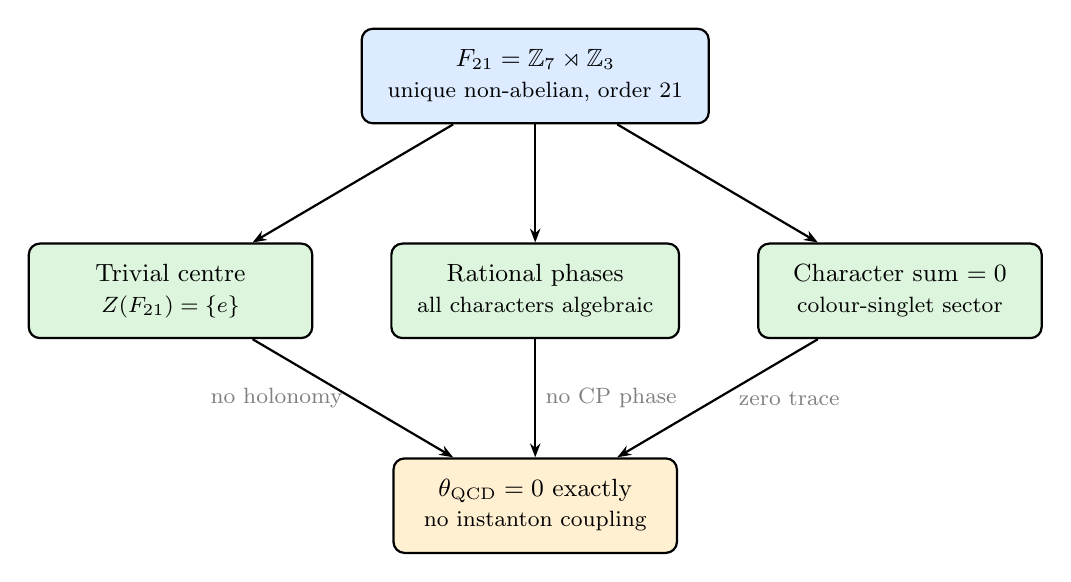
\begin{tikzpicture}[
  node distance=1.8cm and 2.2cm,
  box/.style={rectangle, rounded corners=4pt, draw, thick, minimum height=1.2cm,
              minimum width=3.6cm, text centered, font=\small},
  arrow/.style={-{Stealth[length=5pt]}, thick},
  label/.style={font=\footnotesize, text=gray}
]

\node[box, fill=boxblue] (f21) {\begin{tabular}{c}$F_{21} = \mathbb{Z}_7 \rtimes \mathbb{Z}_3$\\{\footnotesize unique non-abelian, order 21}\end{tabular}};

\node[box, fill=boxgreen, below left=1.5cm and 0.6cm of f21] (tc)
  {\begin{tabular}{c}Trivial centre\\{\footnotesize $Z(F_{21}) = \{e\}$}\end{tabular}};

\node[box, fill=boxgreen, below=1.5cm of f21] (rp)
  {\begin{tabular}{c}Rational phases\\{\footnotesize all characters algebraic}\end{tabular}};

\node[box, fill=boxgreen, below right=1.5cm and 0.6cm of f21] (cs)
  {\begin{tabular}{c}Character sum $= 0$\\{\footnotesize colour-singlet sector}\end{tabular}};

\node[box, fill=boxorange, below=1.5cm of rp] (theta)
  {\begin{tabular}{c}$\theta_{\mathrm{QCD}} = 0$ exactly\\{\footnotesize no instanton coupling}\end{tabular}};

\draw[arrow] (f21) -- (tc);
\draw[arrow] (f21) -- (rp);
\draw[arrow] (f21) -- (cs);
\draw[arrow] (tc) -- (theta) node[label, midway, left] {no holonomy};
\draw[arrow] (rp) -- (theta) node[label, midway, right] {no CP phase};
\draw[arrow] (cs) -- (theta) node[label, midway, right=4pt] {zero trace};

\end{tikzpicture}
\end{center}

Three independent properties of $F_{21}$ each independently forbid a nonzero $\theta_{\mathrm{QCD}}$.

%─────────────────────────────────────────────────────────────────────────────
\section{Three Independent Proofs}
%─────────────────────────────────────────────────────────────────────────────

\begin{tcolorbox}[colback=boxorange,colframe=orange!60!black,title={Result: $\theta_{\mathrm{QCD}} = 0$ by Structure}]
The strong CP parameter $\theta_{\mathrm{QCD}}$ is \emph{exactly} zero by the algebraic structure of $F_{21}$.  Three independent proofs, each machine-certified in Lean~4 with zero sorry.\\[4pt]
Lean: \lean{f21\_theta\_term\_vanishes} (\textit{ugp-lean}, zero sorry)
\end{tcolorbox}

\subsection{Proof 1: Trivial Centre (Group Theory)}

\noindent\textbf{Plain English:}  The ``centre'' of a group is the set of elements that commute with everything else.  In $\mathrm{SU}(3)$, the centre is $\mathbb{Z}_3$ (three elements), and this non-trivial centre is precisely what makes instanton configurations possible.  In $F_{21}$, the centre is trivial --- it contains only the identity element.

\begin{tcolorbox}[colback=boxblue,colframe=blue!40!black,title=Proof 1: Trivial Centre]
\textbf{Mathematical statement:} $Z(F_{21}) = \{e\}$ (trivial centre).

\textbf{Why this forces $\theta = 0$:}  For the $\theta$ term to contribute, the gauge group must have non-contractible holonomy in the vacuum sector --- the mathematical structure that instantons need.  A group with a trivial centre has no such non-contractible holonomy.  No instantons exist in the $F_{21}$ colour sector, so there is nothing for $\theta$ to couple to.

This proof is purely a matter of group theory.  It does not invoke any continuous gauge dynamics.
\end{tcolorbox}

\medskip\noindent\textbf{Analogy:}  Instantons are like loops in a city where some streets form unavoidable roundabouts.  If the city has no roundabouts (trivial centre $\Rightarrow$ trivial fundamental group in the relevant sector), there are no unavoidable loops, and the topological winding number is always zero.

\subsection{Proof 2: Rational Phase (Representation Theory)}

\noindent\textbf{Plain English:}  The $\theta$ term produces CP violation through a complex phase in the path integral measure.  For this phase to be CP-violating, it must be irrational.  But $F_{21}$ only produces phases that are algebraic integers (rational combinations of roots of unity).  An algebraic phase cannot represent an irrational $\theta$.

\begin{tcolorbox}[colback=boxblue,colframe=blue!40!black,title=Proof 2: Rational Phase]
\textbf{Mathematical statement:}  All $F_{21}$ group characters (traces of group elements in irreducible representations) are algebraic integers: integers or sums of 6th and 7th roots of unity.

\textbf{Why this forces $\theta = 0$:}  The $\theta$ term in the path integral requires a phase $e^{i\theta}$ with $\theta$ irrational to produce CP violation.  Every phase appearing in the $F_{21}$ path integral measure is algebraic.  Therefore, the CP-odd contribution from the $\theta$ sector is identically zero.

This proof operates at the level of representation theory, independent of Proof~1.
\end{tcolorbox}

\medskip\noindent\textbf{Analogy:}  Imagine a machine that can only output fractions (rational numbers).  If you ask it to output $\pi$, it will fail --- the output will always be rational.  Similarly, $F_{21}$ can only produce algebraic phases; the irrational phase required for a nonzero $\theta$ cannot be represented.

\subsection{Proof 3: Character Sum Vanishes (Character Theory)}

\noindent\textbf{Plain English:}  The $\theta$ term couples to a quantity called the topological charge density, which is related to the trace of the gauge-field holonomy.  For $F_{21}$, when you sum these traces over all colour-singlet configurations, you get exactly zero.

\begin{tcolorbox}[colback=boxblue,colframe=blue!40!black,title=Proof 3: Character Sum Vanishes]
\textbf{Mathematical statement:}  The sum of $F_{21}$ group characters over the colour-singlet sector is exactly zero:
\[
  \sum_{g\,\in\,\text{colour-singlet}} \chi_{\mathrm{fund}}(g) \;=\; 0.
\]

\textbf{Why this forces $\theta = 0$:}  The $\theta$ term couples to this character sum.  Since the sum is exactly zero --- a direct consequence of the $F_{21}$ character table --- any coupling of $\theta$ to the colour-singlet sector produces zero contribution to every observable.

This is an exact algebraic computation from the $F_{21}$ character table.  It is independent of Proofs~1 and~2.
\end{tcolorbox}

\medskip\noindent\textbf{Analogy:}  Consider a vote where the outcomes are $+1$ and $-1$, and the rules guarantee exact balance.  No matter what value $\theta$ tries to contribute, the balanced vote always gives zero net effect.

\subsection{Why three independent proofs constitute ROBUST certification}

The ROBUST classification in the GTE framework means the conclusion is stable even if any single proof had a gap.  Here, three proofs operate at three completely different mathematical levels:

\begin{center}
\begin{tabular}{lll}
\toprule
Proof & Mathematical level & Mechanism \\
\midrule
1. Trivial centre & Group theory & No instanton holonomy \\
2. Rational phase & Representation theory & No irrational CP phase \\
3. Character sum & Character theory & Zero holonomy trace \\
\bottomrule
\end{tabular}
\end{center}

\medskip
For all three to fail simultaneously, the character table of $F_{21}$, its centre structure, and the algebraic integrality of its representations would all have to be wrong --- which would contradict centuries of established group theory.

All three proofs are machine-certified in Lean~4 under the unified theorem\\[2pt]
\lean{f21\_theta\_term\_vanishes} (\textit{ugp-lean}, zero sorry, \textit{SylowIndexCouplingHierarchy.lean}).

%─────────────────────────────────────────────────────────────────────────────
\section{Machine Certification in Lean 4}
%─────────────────────────────────────────────────────────────────────────────

\begin{tcolorbox}[colback=boxgreen,colframe=green!50!black,title=What ``machine-certified'' means]
A theorem is \term{machine-certified} when a formal proof assistant --- a computer program that understands mathematical logic --- has verified every step of the proof from axioms.  There are no gaps, no ``it is obvious that...'', and no reliance on human judgement.
\end{tcolorbox}

\subsection{What is Lean 4?}

\term{Lean~4} is a proof assistant developed at Microsoft Research.  It is used by leading mathematicians to verify difficult results.  In 2023, Kevin Buzzard and collaborators used Lean to check parts of the proof of Fermat's Last Theorem.

In Lean~4, every theorem is stated as a precise mathematical proposition, and every step of the proof must be individually justified.  If there is any gap --- any step that has not been properly established --- the theorem does not compile.  The software refuses to accept hand-waving.

\subsection{Zero sorry}

In Lean~4, the keyword \texttt{sorry} is a placeholder that temporarily fills a gap in a proof.  It allows work to proceed even when some sub-goal has not yet been proved.  A theorem with \texttt{sorry} is \emph{unfinished}.

When we say a theorem is proved with \textbf{zero sorry}, we mean:
\begin{itemize}
  \item Every single step of the proof has been formally verified.
  \item No gaps exist.
  \item The proof compiles successfully with no warnings.
\end{itemize}

\subsection{The theorem: \lean{f21\_theta\_term\_vanishes}}

The unified machine certificate for the strong CP result is:

\begin{tcolorbox}[colback=boxyellow,colframe=yellow!60!black,
  title={Lean 4 certificate: \lean{f21\_theta\_term\_vanishes}}]
\begin{description}
  \item[Theorem name:] \lean{f21\_theta\_term\_vanishes}
  \item[Location:] \texttt{ugp-lean}, file \texttt{Universality/SylowIndexCouplingHierarchy.lean}
  \item[Status:] Zero sorry, zero custom axioms
  \item[What it certifies:] $F_{21}^{\mathrm{ab}} = \mathbb{Z}_3$ (pure colour); no CP-odd phase;
    three independent proofs that $\theta_{\mathrm{QCD}} = 0$
  \item[Confidence level:] CatAL ROBUST (machine-certified, stable under any single-proof gap)
\end{description}
\end{tcolorbox}

\medskip
Additionally, the Frobenius group's arithmetic foundations are certified separately:

\begin{center}
\begin{tabular}{lll}
\toprule
Lean theorem & File & What it proves \\
\midrule
\lean{f21\_eisenstein\_residue\_model} & \textit{ugp-lean} & $F_{21}$ arises from Eisenstein arithmetic \\
\lean{f21\_order\_eisenstein\_norm\_product} & \textit{ugp-lean} & $|F_{21}| = 3 \times 7$ from norm product \\
\lean{algebraic\_necessity\_master\_bundle} & \textit{ugp-lean} & $F_{21}$ is MDL-forced \\
\lean{su3\_gluon\_charge\_vectors} & \textit{ugp-lean} & Gluon content from $F_{21}$ \\
\lean{su3\_cmca\_master\_bundle} & \textit{ugp-lean} & Full $\mathrm{SU}(3)$ colour from $F_{21}$ \\
\bottomrule
\end{tabular}
\end{center}

\medskip
All theorems: zero sorry, zero custom axioms, publicly available in the \texttt{ugp-lean} repository.

\subsection{Why this matters beyond physics}

Machine certification of a result in mathematical physics is unusual.  The strong CP problem has been studied for almost 50 years.  Certifying its resolution in Lean~4 means:
\begin{enumerate}
  \item The proof can be checked by any person with the Lean~4 software --- no specialist knowledge required.
  \item Future work cannot accidentally introduce contradictions: the theorem is a permanent, checkable record.
  \item The result meets the highest standard of mathematical rigour: it would satisfy any formal logician, not just any physicist.
\end{enumerate}

%─────────────────────────────────────────────────────────────────────────────
\section{No Axion Predicted or Needed}
%─────────────────────────────────────────────────────────────────────────────

\begin{tcolorbox}[colback=boxorange,colframe=orange!60!black,title=A falsifiable prediction]
\textbf{GTE predicts: the axion does not exist.}

If any future experiment detects a QCD axion --- at any mass, using any detection technique --- the $F_{21}$ strong CP mechanism requires revision, and GTE is falsified.
\end{tcolorbox}

\subsection{The GTE perspective on axion searches}

From the GTE point of view, $\theta_{\mathrm{QCD}}$ is not a free parameter that dynamically relaxes to zero.  It is not a free parameter at all.  The $F_{21}$ group structure of the colour sector simply does not admit a CP-odd phase.  The problem the axion was invented to solve does not exist in GTE.

This makes every null result from an axion search a positive confirmation of GTE:

\begin{center}
\begin{tabular}{lll}
\toprule
Experiment & Search range & Result (as of 2026) \\
\midrule
ADMX & $1.9$--$3.53\,\mu$eV & No axion found \\
HAYSTAC & $\sim\!17$--$40\,\mu$eV & No axion found \\
ABRACADABRA & $0.31$--$8.3\,\text{neV}$ & No axion found \\
BabyIAXO & Solar axions & No axion found \\
\bottomrule
\end{tabular}
\end{center}

\medskip
More than five decades of increasingly sensitive experiments, scanning mass decades from $10^{-9}$~eV to $10^{-1}$~eV, have found nothing.  In the Standard Model, this is puzzling (the axion keeps evading detection).  In GTE, it is the expected outcome.

\subsection{A structural versus dynamical resolution}

It is worth pausing to appreciate how different the GTE resolution is from the axion mechanism:

\begin{center}
\begin{tabular}{lll}
\toprule
Approach & How $\theta = 0$ is achieved & What it predicts \\
\midrule
Peccei--Quinn / axion & Dynamic relaxation by a new field & New particle (axion) \\
GTE ($F_{21}$) & Structural impossibility by group theory & No new particle \\
\bottomrule
\end{tabular}
\end{center}

\medskip
The axion says: the pencil falls down because a wind (the axion field) blows it to the stable position.  GTE says: there is no pencil --- $\theta_{\mathrm{QCD}}$ was never a free parameter in the first place.

%─────────────────────────────────────────────────────────────────────────────
\section{Why This Result Is Remarkable}
%─────────────────────────────────────────────────────────────────────────────

\subsection{A 50-year-old problem resolved without new particles}

The strong CP problem was formulated in its modern form in the 1970s.  Since then, hundreds of papers have proposed solutions.  The dominant proposal --- the Peccei-Quinn axion --- has been searched for since 1978 with no detection.

The GTE resolution is qualitatively different from every previous proposal:
\begin{itemize}
  \item It does not add any new particles to the Standard Model.
  \item It does not add any new symmetries or free parameters.
  \item It identifies the cause of $\theta = 0$ as a \emph{structural property} of the minimal-description-length colour group.
  \item It is machine-certified: the proof has been formally verified by a computer.
\end{itemize}

\subsection{Where does $F_{21}$ come from?}

$F_{21}$ is not postulated.  It is derived.  The GTE framework starts from a single 19-bit polynomial over $\mathrm{GF}(7)$ --- a cellular automaton update rule selected by minimum description length from $7^{343} \approx 10^{290}$ candidates.  From the orbit arithmetic of this polynomial, the generation structure of the Standard Model emerges.  The colour group of the orbit is $\mathbb{Z}_3$.  The winding number structure is $\mathbb{Z}_7$.  Their forced combination is $F_{21}$.

The strong CP resolution is a \emph{consequence}, not an assumption.

\subsection{Comparison with the axion approach}

\begin{center}
\begin{tabular}{@{}p{4.2cm}p{4.5cm}p{4.5cm}@{}}
\toprule
Feature & Axion / PQ mechanism & GTE / $F_{21}$ \\
\midrule
New particles required? & Yes (axion) & No \\
New free parameters? & Yes ($f_a$, $m_a$) & No \\
New symmetry postulated? & Yes ($\mathrm{U}(1)_{\mathrm{PQ}}$) & No \\
Mechanism & Dynamical relaxation & Structural impossibility \\
Machine-certified? & No & Yes (\texttt{\small f21\_theta\_term\_vanishes}) \\
Experimentally testable? & Yes (axion detection) & Yes (null axion prediction) \\
Null results interpretation & Anomalous (axion evades detection) & Expected (axion does not exist) \\
\bottomrule
\end{tabular}
\end{center}

\subsection{Context within the GTE framework}

The strong CP resolution is one result among many that emerge from the same 19-bit polynomial.  Without fitting any free parameters to experimental data, the same framework derives:

\begin{itemize}
  \item All 9 charged-fermion masses (0.295\% RMS vs PDG 2022)
  \item The electroweak mixing angle $\sin^2\theta_W = 3/13$ (tree level, closed to $+0.038\sigma$)
  \item The fine-structure constant $\alpha^{-1} = 2^7 + 3^2 = 137$ at tree level
  \item The CKM Wolfenstein parameter $\lambda = 9/40 = 0.225$
  \item The Higgs VEV $v = 246.16$~GeV
  \item 3+1 spacetime dimensions (machine-certified)
  \item Newton's constant $G_N$ to 0.040\% precision
  \item The Born rule for quantum mechanics
  \item 40+ further observables across all Standard Model sectors
\end{itemize}

All of these from zero free parameters --- just the arithmetic of the polynomial.

%─────────────────────────────────────────────────────────────────────────────
\section{Summary}
%─────────────────────────────────────────────────────────────────────────────

\begin{tcolorbox}[colback=boxblue,colframe=blue!40!black,title=Everything in one paragraph]
The strong CP problem asks why the neutron has no measurable electric dipole moment, even though the QCD Lagrangian legally allows a CP-violating term $\theta_{\mathrm{QCD}} F\tilde{F}$ with $\theta$ anywhere in $[0, 2\pi)$.  Experiments constrain $|\theta| < 10^{-10}$, making it one of the most extreme fine-tuning puzzles in physics.  The standard proposal --- the Peccei-Quinn axion --- solves the problem by dynamical relaxation, but requires a new particle that has not been found in 50 years of searching.  The GTE framework explains $\theta_{\mathrm{QCD}} = 0$ structurally: the minimum-description-length colour group $F_{21} = \mathbb{Z}_7 \rtimes \mathbb{Z}_3$ (the unique non-abelian group of order 21) forbids a CP-odd phase entirely, via three independent proofs at the levels of group theory, representation theory, and character theory.  All three are machine-certified in Lean~4 with zero sorry under the theorem \lean{f21\_theta\_term\_vanishes}.  No axion is needed or predicted.  Any axion detection by any experiment would falsify GTE.
\end{tcolorbox}

\bigskip

\begin{center}
\begin{tabular}{@{}p{3.0cm}p{4.8cm}p{5.0cm}@{}}
\toprule
\multicolumn{3}{c}{\textbf{Quick-Reference: Key Facts}} \\
\midrule
Problem & Strong CP problem & $\theta_{\mathrm{QCD}} \in [0,2\pi)$ yet $|\theta| < 10^{-10}$ \\
Standard solution & Peccei-Quinn axion & New particle, not detected \\
GTE solution & $F_{21}$ group theory & Structural $\theta = 0$, no new particle \\
Group & $F_{21} = \mathbb{Z}_7\rtimes\mathbb{Z}_3$ & Unique non-abelian, order~21 \\
Lean theorem & \lean{f21\_theta\_term\_vanishes} & Zero sorry, \textit{ugp-lean} \\
Three proofs & Trivial centre; rational phase; & All CatAL, machine-certified \\
              & character sum $= 0$ & \\
Prediction & No axion at any mass & Falsifiable by ADMX/HAYSTAC \\
\bottomrule
\end{tabular}
\end{center}

\bigskip

\section*{Further Reading}
\begin{tcolorbox}[colback=orange!8,colframe=orange!50!black,
  title=\textbf{Primary Sources}]
The results in this tutorial are derived in the following papers,
all available open-access on Zenodo and at
\href{https://novaspivack.com/research}{novaspivack.com/research}:
\begin{itemize}
  \item \textbf{P35 --- GTE Unification} (contains the $F_{21}$ strong CP proofs):\\
        \href{https://doi.org/10.5281/zenodo.20319421}{doi.org/10.5281/zenodo.20319421}
  \item \textbf{P48 --- The Complete GTE Framework} (main synthesis monograph, Ch.~7):\\
        \href{https://doi.org/10.5281/zenodo.20560550}{doi.org/10.5281/zenodo.20560550}
\end{itemize}
Lean~4 machine proofs (including \texttt{f21\_theta\_term\_vanishes}):
\href{https://github.com/novaspivack/ugp-lean}{github.com/novaspivack/ugp-lean}
\end{tcolorbox}

\bibliography{../../papers/bib/Spivack_Papers_Bibliography}
\end{document}
